% This file was created with tikzplotlib v0.10.1.
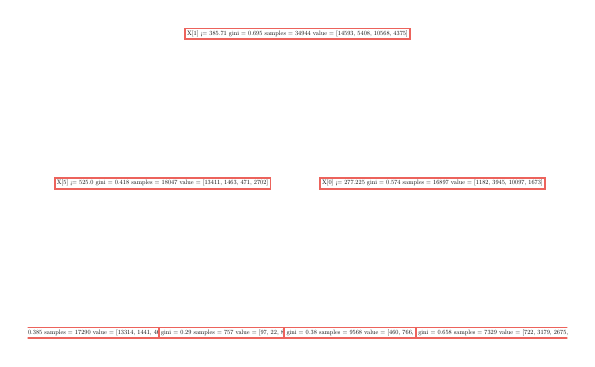
\begin{tikzpicture}

\definecolor{darkgray176}{RGB}{176,176,176}
\definecolor{tomato2369992}{RGB}{236,99,92}

\begin{axis}[
hide x axis,
hide y axis,
tick align=outside,
tick pos=left,
x grid style={darkgray176},
xmin=0, xmax=1,
xtick style={color=black},
y grid style={darkgray176},
ymin=0, ymax=1,
ytick style={color=black}
]
\draw (axis cs:0.125,0.166666666666667) node[
  scale=0.227406454379758,
  fill=white,
  draw=tomato2369992,
  line width=0.6pt,
  inner sep=3.6pt,
  text=black,
  rotate=0.0,
  align=center
]{gini = 0.385
samples = 17290
value = [13314, 1441, 463, 2072]};
\draw (axis cs:0.375,0.166666666666667) node[
  scale=0.227406454379758,
  fill=white,
  draw=tomato2369992,
  line width=0.6pt,
  inner sep=3.6pt,
  text=black,
  rotate=0.0,
  align=center
]{gini = 0.29
samples = 757
value = [97, 22, 8, 630]};
\draw (axis cs:0.625,0.166666666666667) node[
  scale=0.227406454379758,
  fill=white,
  draw=tomato2369992,
  line width=0.6pt,
  inner sep=3.6pt,
  text=black,
  rotate=0.0,
  align=center
]{gini = 0.38
samples = 9568
value = [460, 766, 7422, 920]};
\draw (axis cs:0.875,0.166666666666667) node[
  scale=0.227406454379758,
  fill=white,
  draw=tomato2369992,
  line width=0.6pt,
  inner sep=3.6pt,
  text=black,
  rotate=0.0,
  align=center
]{gini = 0.658
samples = 7329
value = [722, 3179, 2675, 753]};
\draw (axis cs:0.25,0.5) node[
  scale=0.227406454379758,
  fill=white,
  draw=tomato2369992,
  line width=0.6pt,
  inner sep=3.6pt,
  text=black,
  rotate=0.0,
  align=center
]{X[5] <= 525.0
gini = 0.418
samples = 18047
value = [13411, 1463, 471, 2702]};
\draw (axis cs:0.75,0.5) node[
  scale=0.227406454379758,
  fill=white,
  draw=tomato2369992,
  line width=0.6pt,
  inner sep=3.6pt,
  text=black,
  rotate=0.0,
  align=center
]{X[0] <= 277.225
gini = 0.574
samples = 16897
value = [1182, 3945, 10097, 1673]};
\draw (axis cs:0.5,0.833333333333333) node[
  scale=0.227406454379758,
  fill=white,
  draw=tomato2369992,
  line width=0.6pt,
  inner sep=3.6pt,
  text=black,
  rotate=0.0,
  align=center
]{X[1] <= 385.71
gini = 0.695
samples = 34944
value = [14593, 5408, 10568, 4375]};
\end{axis}

\end{tikzpicture}
